\documentclass[10pt]{article}

\usepackage[utf8]{inputenc}
\usepackage{floatrow}

\usepackage{algorithm, algpseudocode}
\let\oldReturn\Return
\renewcommand{\Return}{\State\oldReturn}
\newcommand{\N}{\mathbb{N}}
\newcommand{\R}{\mathbb{R}}
\usepackage[T1]{fontenc}
\usepackage{enumitem}
\usepackage{hyperref}
\usepackage{scrextend}
\usepackage{amsmath}
\usepackage{amsfonts}
\usepackage{stmaryrd}
\usepackage{graphicx}
\usepackage{color}
\usepackage{listings}
\usepackage{wrapfig}
\usepackage[hmargin=1.25in,vmargin=1.25in]{geometry}

%title setup
\title{TD1 : l'ordonnanceur du noyau Linux}
\author{Romain PEREIRA}
\date{25/10/2018}

% table of contents setup
\renewcommand{\contentsname}{Sommaire}
\usepackage{etoolbox}
\patchcmd{\thebibliography}{\section*{\refname}}{}{}{}

\usepackage[utf8]{inputenc}
\usepackage[T1]{fontenc}
\usepackage[frenchb]{babel}

\setlength{\parindent}{0cm}
\setlength{\parskip}{1ex plus 0.5ex minus 0.2ex}
\newcommand{\hsp}{\hspace{20pt}}
\newcommand{\HRule}{\rule{\linewidth}{0.5mm}}

\hypersetup{
    colorlinks,
    citecolor=black,
    filecolor=black,
    linkcolor=blue,
    urlcolor=red
}

\lstset{language=C,
                basicstyle=\ttfamily,
                keywordstyle=\color{blue}\ttfamily,
                stringstyle=\color{red}\ttfamily,
                commentstyle=\color{cyan}\ttfamily,
                morecomment=[l][\color{magenta}]{\#}
}

\lstdefinelanguage{Markdown}{}

\begin{document}
    
    \begin{titlepage}
        \begin{sffamily}
            \begin{center}

                \begin{figure}[h!]
                    
\includegraphics[width=6cm]{ensiie.jpeg}
                \end{figure}

                \HRule \\[0.4cm]
                { \huge \bfseries Architecture d'un système d'exploitation\\[0.4cm] }
                \HRule \\[2.0cm]
                
                { \huge \bfseries TD2\\[0.5cm] }

                \textsc{\Large L'ordonnanceur du noyau Linux}\\[2.0cm]

                \vfill
                \begin{minipage}{0.4\textwidth}
                    \begin{flushleft} \large
                        \emph{Etudiant:} Romain \textsc{Pereira}\\
                    \end{flushleft}
                \end{minipage}
                \begin{minipage}{0.4\textwidth}
                    \begin{flushright} \large
                        \emph{Encadrants:}  M. \textsc{Loussert}\\
                                            M. \textsc{Taboada}
                    \end{flushright}
                \end{minipage}
                \\[2.0cm]
                {\large 25/10/2018}
            \end{center}
        \end{sffamily}
    \end{titlepage}
    
    \maketitle
    \tableofcontents
    \section{Préambule}
    
    Le but de ce TP est de comprendre le fonctionnement d'un ordonnanceur, en étudiant l'ordonnanceur du noyau Linux.

    \newpage
    \section{Fonctionnement de l'ordonnanceur}
        \paragraph{Q.1}
        Nos ordinateurs de bureau dispose généralement d'un seul processeur (avec 1, 2, 4 ou 8 coeurs d'execution).
        Le processeur est le seul point d'execution possible pour les processus.
        
        Lorsque plusieurs processus s'execute sur le même processeur, il faut donc qu'il y ait un méchanisme de partage du processeur.
    
        C'est la fonction principale de l'ordonnanceur.
        Il choisit dans quel ordre, et pendant combien de temps les processus peuvent être executé sur le processeur.
                        
        L'execution de l'ordonnanceur peut avoir lieu pour répondre aux problèmes suivants:
        
        \begin{itemize}
            \item Lorsqu'un processus se clone (appel $fork()$) : lequel du père ou du fils a la priorité d'éxecution?
            \item Lorsque le processus courant s'arrête : quel processus doit prendre la main ensuite
            \item Lorsqu'un processus bloque sur une entrée/sortie, ou qu'il est en attente :
            doit t'il continuer de bloquer le processeur alors qu'il ne travaille pas?
            \item Lorsqu'une entrée/sortie est interrompu : peut être que le processus a fini son job,
            ou bien c'est un signal indiquant qu'un processus précèdemment en attente entrée/sortie
            peut maintenant effectué son travail.
        \end{itemize}
        
        
        Aussi, on distingue 2 grandes politiques décidant de l'execution de l'ordonnanceur.
        \begin{itemize}
            \item \textbf{préemptif} : l'ordonnanceur peut stopper l'éxecution d'un processus,
            et donner la main sur le CPU à un autre processus.
            \item \textbf{non-préemptif} : l'ordonnanceur ne tourne que si le processus utilisateur
            s'arrête, bloque, ou demande explicitement à changer de processus.
            Si le processus ne rends pas la main pendant 100 ans, l'ordonanneur attendra impassiblement pendant 100 ans.

        \end{itemize}

        
        \paragraph{Q.2}
        La fonction \textit{sched\_yield} passe la main sur le processeur d'un processus à un autre
        (ou d'un processus vers lui même s'il reste le plus 'prioritaire').
        
        S'il n'y a pas d'autre processus devant être executer, cette fonction s'arrête.
        
        \paragraph{Q.3}
        Code modifié
        \lstset{language=C}
\begin{lstlisting}[frame=single]
[...]
printk("current=%p\n", current);
schedule();
printk("current=%p\n", current);
[...]
\end{lstlisting}

        Compilation de l'image linux modifié et déploiement
\lstset{language=bash}
\begin{lstlisting}[frame=single]
cd ~/debian_kernel/linux-4.9.30/
make bindeb-pkg
dpkg -i ../linux-image-4.9.30_4.9.30-2_amd64.deb
reboot
\end{lstlisting}

Programme utilisateur 'main.c'
\lstset{language=C}
\begin{lstlisting}[frame=single]
int main() {
    sched_yield();
    return 0;
}
\end{lstlisting}

Compile et lance le programme utilisateur
\begin{lstlisting}[frame=single]
gcc main.c
./a.out
dmesg
\end{lstlisting}

Sortie dmesg
\begin{lstlisting}[frame=single]
[  170.029953] current=ffff9337bbe47140
[  170.029956] current=ffff9337bbe47140
\end{lstlisting}

=> Le pointeur 'current' reste inchangé
Ceci est dû au fait que peu de processus tourne sur la machine virtuelle.
Le processus prioritaire reste le même entre 2 appels de $schedule()$

En lançant d'autres processus sur la machine, la valeur du pointeur aurait changé


\paragraph{Q.4}
On génère d'abord les 'ctags' pour naviguer plus facilement dans le code source.

\lstset{language=bash}
\begin{lstlisting}[frame=single]
cd ~/debian_kernel/linux-4.9.30/
ctags -R .
\end{lstlisting}


Lecture de 'core.c'
\lstset{language=C}
\begin{lstlisting}[frame=single]
ligne  profondeur/schedule()  execution
4898  0  schedule();

3454  1  sched_submit_work(task);
3438  2  ...

//debut boucle : desactive le préemption
3456  1  preempt_disable();

3457  1  __schedule(false);
3342  2  cpu_rq(); // recuperes la 'run queue' du CPU
3343  2  prev = rq->curr; // enregistre le processus courant dans la run queue
3391  2  next = pick_next_task(rq, prev, cookie); // recuperes la task suivante

// réactive la préemption
3457  1  sched_preempt_enable_no_resched();

3459  1  need_resched();
// tant que 'need_resched()' renvoit 'vrai',
// on boucle sur partir de preempt_disable()
\end{lstlisting}
        
\paragraph{Q.5} La fonction principal de l'ordonnanceur est 'schedule()'

\lstset{language=C}
\begin{lstlisting}[frame=single]
// choisit le prochain processus à être executé
// avant l'appel de cette fonction, un processus tourne
schedule();
// apres l'appel, un autre processus peut tourner
\end{lstlisting}
        
\paragraph{Q.6}
La préemption est un mecanisme d'ordonnancement.

Il donne à chaque processus à un temps d'execution maximal. \label{preempt}
L'ordonnanceur est executé à intervalle régulier, et détermine le prochain prochain
processus qui doit être executé sur le prochain 'créneau'.

La préemption est desactivé dans l'ordonnanceur, car le code de l'ordonnanceur à la priorité d'execution sur le CPU.
Il ne doit pas être interrompu dans son execution.

De plus, la desactivation de la préemption permet d'éviter de compatibiliser
le temps passé par le processus dans le code de l'ordonnanceur.

 \paragraph{Q.7}
 La 'run-queue' est une file de priorité. Elle stocke les processus par ordre de priorité d'éxecution.
 A chaque processeur est associé une run-queue.
 
 La run-queue est verouillé au début de la fonction \textit{schedule} (alors que le processus 'prev' vient de finir son créneau d'execution)
 
 Ensuite, le prochain processus devant être executé est élu par l'ordonnanceur : c'est le processus 'next'
 
 Une fois l'election terminé, le verrou de la run-queue est retiré et le processus 'next' commence son execution.
 
 Ce verrou sur la run-queue permet donc de ne pas modifier la priorité des processus pendant l'éléction.
 Une fois l'election terminé, le processus 'next' libère ce verrou pour que la priorité des processus puissent être mis à jour par la suite.
 
\paragraph{Q.8} ligne 3258 core.c
\lstset{language=C}
\begin{lstlisting}[frame=single]
struct task_struct *pick_next_task (struct rq *rq,
				    struct task_struct *prev,
				    struct pin_cookie cookie);
\end{lstlisting}

  \newpage
 \paragraph{Q.9}
    Description brève du fonctionnement de l'ordonnanceur
    
    \begin{figure}[h!]
        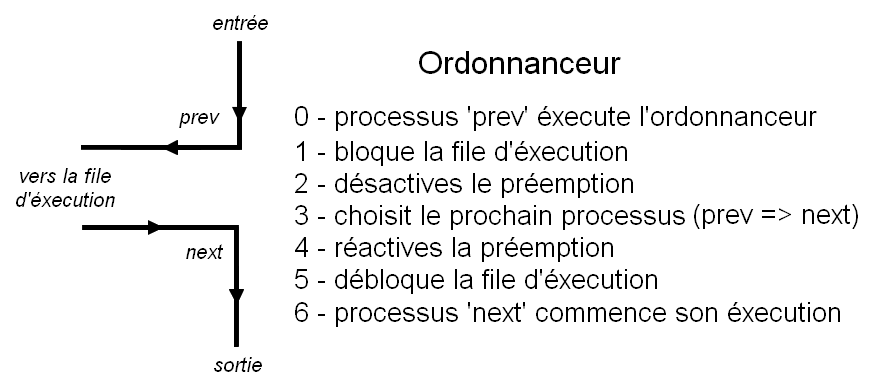
\includegraphics[width=12cm]{q9.png}
    \end{figure}

 \paragraph{Q.10}
 La fonction $context\_switch$ se trouve à la ligne 2862 du fichier 'core.c'.
 Elle est declaré en $\_\_always\_inline$, ce qui signifie que le code de cette fonction doit être duppliqué par le compilateur,
 et ré-insérer dans le binaire executable à chaque appel vers cette fonction (voir \ref{inlinefunc} )
 
 Cette fonction rétablie l'état du processus sur le processeur, état dans lequel il avait été stoppé lors de son dernier créneau d'execution (ou dans un nouvel état si c'est un nouveau processus).

\newpage
\section{Abstractions de l'ordonnanceur}
 \paragraph{Q.12}
 L'usage de pointeur de fonctions permet de relier l'ordonnanceur à des algorithmes d'ordonnancement.
 
 La structure $struct sched\_class$ définit toutes les fonctions qu'un algorithme d'ordonnancement doit implémenter.
 
 Il suffit d'initialiser cette structure avec des implémentations des fonctions de l'algorithme, et l'ordonnanceur l'executera

 Dans le fichire core.c, c'est le CFS (Completely Fair Scheduling) qui est utilisé

\lstset{language=C}
\begin{lstlisting}[frame=single]
      /*
9023  * All the scheduling class methods:
9024  */ 
9025 const struct sched_class fair_sched_class = {
9026     .next           = &idle_sched_class,
9027     .enqueue_task       = enqueue_task_fair,
9028     .dequeue_task       = dequeue_task_fair,
9029     .yield_task     = yield_task_fair,
9030     .yield_to_task      = yield_to_task_fair,
9031     [...] 
\end{lstlisting}

  \paragraph{Q.13}
  Voici quelques algorithme d'ordonnancement du noyau Linux.
  
    \begin{itemize}
        \item \textbf{SCHED\_NORMAL : Completely Fair Scheduling (CFS)} est l'algorithme utilisé par défaut sur de très nombreuses distributions Linux.
        Il est detaillé en \ref{cfs}
        \item \textbf{SCHED\_DEADLINE : Deadline Scheduler}
        \item \textbf{SCHED\_RR : Round-Robin Scheduling}
        \item \textbf{SCHED\_FIFO : First in, first out} : c'est l'algorithme le plus simple envisageable.
        Les processus demandent du temps d'éxecution sur le CPU.
        Ces demandes sont placés dans une file FIFO (les processus sont éxecutés
        dans l'ordre dans lequelle ils ont demandé le CPU : 1er arrivé, 1er servi).
        \item \textbf{Brain Fuck Scheduler (BFS) \ref{bfssched}} est utilisé par défaut dans quelques distributions.
        Il a été proposé comme une alternative plus légère au CFS (avec nombre plus faible d'heuristiques et de paramètres à ajuster).
    \end{itemize}

robably the simplest of all scheduling algorithms ever devised is nonpreemp-
tive first-come, first-served. With this algorithm, processes are assigned the CPU
in the order they request it. Basically, there is a single queue of ready processes.
When the first job enters the system from the outside in the morning, it is started
immediately and allowed to run as long as it wants to. It is not interrupted because
it has run too long. As other jobs come in, they are put onto the end of the queue.
When the running process blocks, the first process on the queue is run next. When
a blocked process becomes ready, like a newly arrived job, it is put on the end of
the queue, behind all waiting processes.SEC. 2.4
157
SCHEDULING
The great strength of this algorithm is that it is easy to understand and equally
easy to program. It is also fair in the same sense that allocating scarce concert
tickets or brand-new iPhones to people who are willing to stand on line starting at
2 A . M . is fair. With this algorithm, a single linked list keeps track of all ready proc-
esses. Picking a process to run just requires removing one from the front of the
queue. Adding a new job or unblocked process just requires attaching it to the end
of the queue. What could be simpler to understand and implement?
Unfortunately, first-come, first-served also has a powerful disadvantage. Sup-
pose there is one compute-bound process that runs


\newpage
\section{Completely Fair Scheduling (CFS)}\label{cfs}
  \paragraph{Q.14} Il est implémenté dans le fichier \textbf{kernel/sched/fair.c}

  \paragraph{Q.15} Cet algorithme se base sur les 'red-black tree' (arbre binaire bicolore \ref{rbtree})

  \paragraph{Q.16} Cette algorithme est décrit avec détail dans l'ouvrage \ref{modernos} , page 749.
  
  L'algorithme CFS stocke les processus dans une file de priorité ayant la structure d'un red-black tree (appelé 'run-queue').
  
  Ils sont positionnés dans l'arbre en fonction du temps qu'ils ont passé à s'éxecuter sur le CPU (appelé 'vruntime', précision en nanosecondes).
  
  Les sommets avec le plus petit 'vruntime' sont placés 'à gauche' dans l'arbre, et ceux avec plus de 'vruntime', 'à droite'.
  
  \textbf{étape 1} - Le CFS sort de l'arbre le processus qui a le plus petit 'vruntime' (celui le plus 'à gauche' dans l'arbre).
  Ce processus est mis en éxecution sur le CPU.

  \textbf{étape 2} Périodiquement, le CFS incrémente le 'vruntime' du processus en cours, en fonction du temps
  qu'il a déjà passé à s'éxecuter.
  
  \textbf{étape 3.1} Si le 'vruntime' du processus en cours est plus petit que le minimum de l'arbre, son execution continu.
  
  \textbf{étape 3.2} Sinon, il est inséré dans l'arbre à l'endroit approrié, puis retour à \textbf{l'étape 1}.
  
  Pour prendre en compte la priorité des processus, le CFS incrémente plus ou moins
  vite le 'vruntime' des processus (au cours de \textbf{l'étape 1})
  
  Pour les processus avec une priorité plus basse, le temps s'écoule plus vite.
  Cela permet de passer plus rapidement à \textbf{l'étape 3.2} pour ces processus (c'est à dire de stopper son éxecution, et passer au processus suivant).
  
  L'insertion d'un processus dans l'arbre se fait en $O(log(n))$, avec 'n' le nombre de processus actif dans le système.
  Dans les systèmes actuelles, on ne dépasse généralement pas 100 processus actifs ($log(100) \simeq 6.7$).
  
  Aussi, cette file d'éxecution en 'red-black tree' ne contient que les processus pouvant être éxecuté.
  
  Les processus bloquant, en attente d'un signal (type I/O), sont placés dans une file d'attente concurrante ('wait-queue').
  Lorsqu'un évènement les débloque et qu'ils peuvent être éxecuté, ils sont alors placés dans la 'run-queue'.

    \newpage
    \section{Références}
    \begin{thebibliography}{}

        \bibitem{modernos}\label{modernos}
        Modern Operating Systems - Andrew S. Tanenbaum, Herbert Bos (page 149-166 et 749)\newline
        \href{https://github.com/concerttttt/books/blob/master/Modern Operating Systems 4th Edition--Andrew Tanenbaum.pdf}
        {\textit{https://github.com/concerttttt/books/}}\newline
	
        \bibitem{rbtree}\label{rbtree}
        Arbre bicolore - Wikipédia\newline
        \href{https://fr.wikipedia.org/wiki/Arbre\_bicolore}
        {\textit{https://fr.wikipedia.org/wiki/Arbre\_bicolore}}\newline
	
        \bibitem{inlinefunc}\label{inlinefunc}
        Inlining in Linux - Linux Kernel Documentation\newline
        \href{https://www.kernel.org/doc/local/inline.html}
        {\textit{https://www.kernel.org/doc/local/inline.html}}\newline
               
        \bibitem{{bfssched}}\label{bfssched}
        Brain\_Fuck\_Scheduler - Wikipédia\newline
        \href{https://en.wikipedia.org/wiki/Brain\_Fuck\_Scheduler}
        {\textit{https://en.wikipedia.org/wiki/Brain\_Fuck\_Scheduler}}\newline

        
    \end{thebibliography}
    
\end{document}
